Cette partie présentera les différents algorithmes qui ont été choisis pour générer des anaglyphes dans le logiciel.

\subsubsection{La génération des anaglyphes et ses défauts}
	L'anaglyphe est une image issue d'un traitement particulier sur deux prises de vue stéréoscopiques et qui nécessite des lunettes spécifiques composées d'un filtre rouge (ou magenta ou jaune) pour un \oe il et cyan (respectivement vert ou bleu) pour l'autre. 
	
	La génération des anaglyphes passe par trois étapes essentiellement. Tous d'abord, une prise de vue stéréoscopique d'une scène 3D avec les deux points de vue éloignés d'une distance proche de celle entre les yeux, de manière à obtenir une vue pour chaque \oe il, est nécessaire. Ensuite, un traitement est opéré sur ces deux images, avec au minimum l'application de deux filtres rouge et cyan (ou deux autres couleurs correspondants à celles des lunettes). Finalement, les deux images résultantes sont superposées pour n'obtenir qu'une seule image qui pourra être visionnée à travers les lunettes avec une impression de trois dimensions.
	
	Les algorithmes de génération des anaglyphes proposent des traitements d'image différents (deuxième étape) ayant pour but d'améliorer la qualité des anaglyphes. Un critère important pour juger de la qualité des anaglyphes est l'absence d'artefacts. Il s'agit de perceptions d'un phénomène de diaphonie qui est le résultat d'une mauvaise séparation des deux vues (un \oe il perçoit un détail de la vue destiné à l'autre \oe il), et dégradent l'impression de trois dimensions. %parler des rivalités binoculaire..? 

	Cependant, aucun algorithme ne peut être parfait, comme il est expliqué dans l'article d' Andrew J. Woods et Chris R. Harris \cite{anaglypheDefaut}  : la qualité de l'anaglyphe dépend de l'image, des lunettes employées et du support affichant l'image (l'article traite principalement les écrans mais il en va de même pour des anaglyphes imprimés avec le choix du papier). Hormis les lunettes, les deux autres facteurs ont toujours été problématiques pour le traitement d'image en général.  
	
	Pour obtenir des algorithmes très performants, il faudrait prendre en compte tous ces facteurs et adapter au cas par cas. En effet, étant donné que les différentes caractéristiques (luminosité, résolution,) varient pour chaque écran, obtenir une même couleur sur deux écrans distincts (produits par des entreprises différentes) suppose un calibrage au préalable ou l'utilisation d'une palette de couleur limitée. Ainsi, les techniques employés dans le domaine de recherche de la génération des anaglyphes restent très souvent basées sur des connaissances empiriques.
		
	Nous avons choisi d'implémenter deux méthodes qui permettent d'obtenir des images de qualité différentes, pour que l'utilisateur puisse choisir pour chaque donnée entrée l'algortihme qui rendra l'anaglyphe de meilleure qualité. %phrase a reprendre...
	  
\subsubsection{La méthode Photoshop}
	Le premier algorithme implémenté est le plus basique : c'est la méthode dite Photoshop qui se contente d'appliquer les deux filtres de couleur sans réaliser d'autres traitements d'image. Cette méthode est décrite dans l'article rédigé par W. Alkhadour, S. Ipson, J. Zraqou, R. Qahwaji et J. Haigh \cite{steteroAnaglyph}. Un exemple de rendu obtenu avec cette méthode est présenté dans la Figure \ref{fig:photoshop}.
		
	En pratique, ce ne sont pas des filtres de couleur qui sont appliqués, mais pour chaque image seules les composantes rouges pour l'une et les composantes bleues et vertes pour l'autre sont recupérées et restituées. Ces deux images sont ensuite "superposées", c'est-à-dire que celles-ci sont parcourues et pour chaque pixel les composantes en couleur (RGB) sont récupérées, additionnées deux à deux et réinsérées dans les canaux de couleurs du pixel correspondant dans l'image résultat. %phrase à simplifier ?
	
\begin{figure}[h]
	\centering
	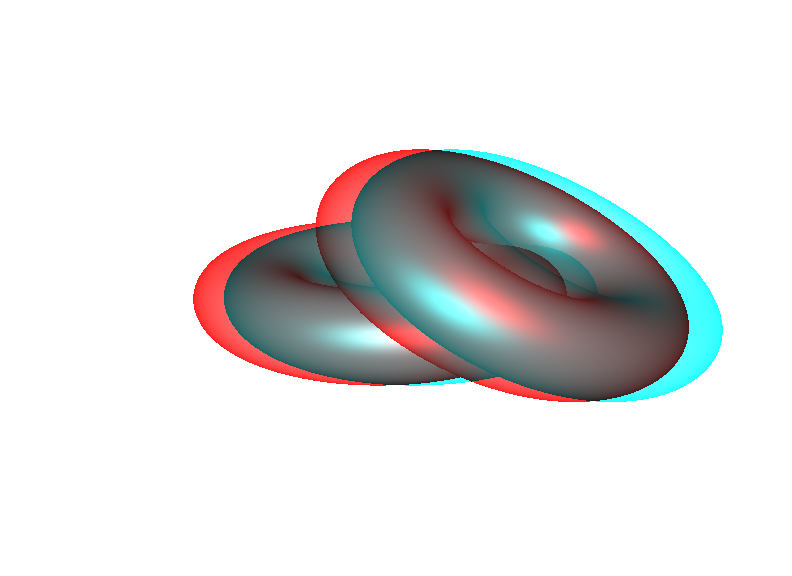
\includegraphics[scale=0.3]{photoshop.png}
	\caption{\label{fig:photoshop} Anaglyphe obtenu avec la méthode Photoshop \protect}
\end{figure}
		
% %ne pas oublier de mettre une référence à l'article

	Au niveau du résultat, on constate la présence de quelques d'artefacts notamment à l'écran sur des formes complexes avec beaucoup de détail. A l'impression, le rendu est plus agréable avec moins d'artefact. Globalement, cette méthode permet de voir rapidement la 3D sans trop fatiguer l'oeil.
%	--> la méthode la plus simple mais la qualité en couleur est mauvaise et il y a un peu de artefact
\subsubsection{La méthode des moindres carrés avec correction gamma}
%gamma -> prend en compte le support : écran
	Le deuxième algorithme implémenté est basé sur la méthode des moindres carrés présentée dans l'article \cite{algoDubois} par Eric Dubois. Dans cet article, comme David Romeuf l'explique \cite{explicationAlgoDubois} l'approche consiste à prendre en compte le spectre d'absorption des filtres des lunettes, la densité spectrale des sources primaires des écrans d'ordinateur et la sensibilité spectrale de l'œil humain, pour reproduire au mieux une image anaglyphe dont les couleurs sont proches de celles contenues dans l'image originale. Un exemple de rendu obtenu avec cette méthode est présenté dans la Figure \ref{fig:moindresCarres}.
	
	L'ensemble des couleurs visibles sur l'écran à travers les lunettes étant un sous ensemble de celui de l'écran, une transformation particulière est nécessaire et c'est pour cette raison que les moindres carrés interviennent dans la projection pour minimiser la distance entre les deux couleurs (celle obtenue et l'originale) dans le diagramme colorimétrique.
	
	L'algorithme implémenté met en \oe uvre une partie de la méthode décrite plus précisément dans cet article par Eric Dubois \cite{algoMoindreCarres} : notre algorithme utilise les matrices issues du calcul par projection avec la méthode des moindres carrés, et une correction gamma mais ne modifie pas la saturation.
	
	La correction gamma permet d'augmenter la luminosité, appliquée aux anaglyphes rouge-cyan le rouge est plus visible et l'impression de trois dimensions est renforcée. Cependant, l'augmentation de la luminosité implique une réduction des contrastes et peut résulter en une image avec les détails peu soignés.

\begin{figure}[h]
	\centering
	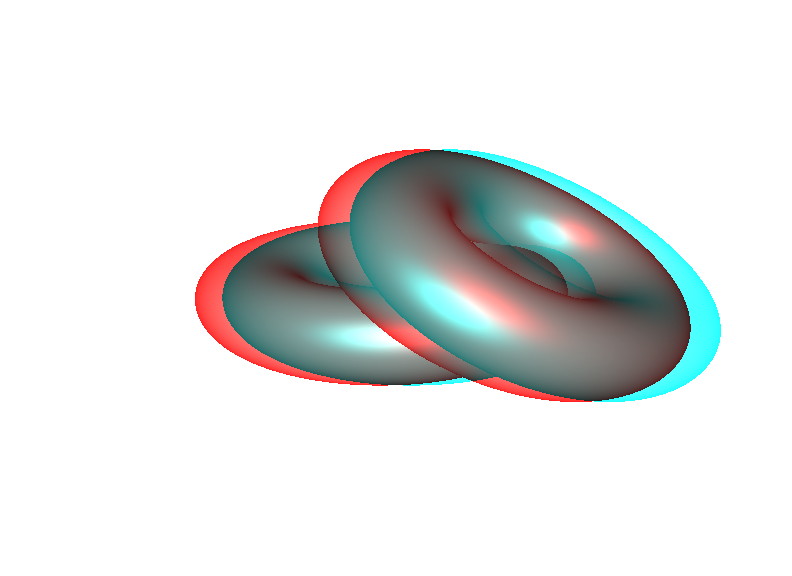
\includegraphics[scale=0.3]{moindreCarres.png}
	\caption{\label{fig:moindresCarres} Anaglyphe obtenu avec la méthode des moindres carrés \protect}
\end{figure}
	
	On constate qu'il y a très peu d'artefact et la 3D est de meilleure qualité que pour la méthode Photoshop. Toutefois, la qualité en couleur est légèrement perdue et les détails de l'image sont peu visibles. 
	

\subsubsection{Comparaison des différents algorithmes}

En comparant les algorithmes, il semblerait que pour une scène contenant un ou des objets simples % %REF FIGURE DOGNUTS
, la méthode Photoshop soit la plus efficace avec une impression de trois dimensions bien visible et peu d'artefacts. En ce qui concerne les objets plus complexes tels que % %REF FIGURE HAPPY
les détails se perdent avec la méthode Photoshop alors qu'avec la méthode de Dubois tous les détails sont conservés dans l'image anaglyphe résultat. 
% %dognuts photshop & dubois
% %happy photoshop & happy dubois 

Cependant, après plusieurs comparaisons des images (et ce par différentes personnes) la correction gamma employée dans la méthode de Dubois fatiguerait plus vite les yeux que la méthode Photshop.

Par ailleurs, il a aussi été observé que l'utilisation de l'anti-aliasing combiné aux algorithmes de génération d'anaglyphe, peut permettre de renforcer l'impression de trois dimensions dans certains cas. Cependant, l'anti-aliasing aura aussi pour effet de perdre beaucoup de détails comme la figure REF le montre avec un comparatif d'algorithmes avec et sans utlisation d'anti-aliasing. 
% %happy anti-aliasing dubois &  happy dubois (sans anti-aliasing)

Un autre point remarqué lors des différentes observations est la fatigue des yeux provoquée par la vision des anaglyphes et celle-ci varie selon les algorithmes. Il semblerait que l'algorithme de Dubois fatiguerait plus vite les yeux et que l'utilisation d'anti-aliasing rendrait la perception plus agréable et donc moins fatiguante. 
%l'algo dubois avec saturation -> la diminution de saturation, atténue trop les couleurs : moins bonne 3D mais moins fatiguant pour les yeux 

\subsubsection{L'impression des anaglyphes}
Dans ce projet, les anaglyphes générés par le logiciel étaient destinés à être visionnés sur écran mais aussi être imprimés sur papier. Le système de colorimétrie d'une imprimante est en CMJN (Cyan Magenta Jaune Noir) et son ensemble de couleur est plus réduit que celui des écrans. 

% %INSERER Diagramme comparatif pour illustrer ?

Par conséquent, le problème pour l'impression réside tout d'abord en la conversion du système RVB au CMJN. Tout comme l'algortihme de Dubois avec la méthode des moindres carrés \cite{algoDubois}, il faudrait pouvoir convertir en CMJN en essayant d'obtenir une couleur qui sera la plus proche possible de celle en RVB. 

Lorsque ce problème a été exposé en réunion avec les clients, il nous a été spécifié que nous n'avions pas besoin d'implémenter des méthodes pour améliorer l'impression. 

Par ailleurs, la conversion n'est pas le seul problème puisque comme expliqué avec l'article Andrew J. Woods et Chris R. Harris \cite{anaglypheDefaut}, le support d'affichage est aussi important : dans ce cas, le type de papier rentre aussi en compte dans la qualité de l'anaglyphe.

Finalement, la qualité de l'impression d'un anaglyphe dépendant trop des réglages en amont et du matériel utilisé, aucun algorithme particuliers n'a été implémenté. Cependant, nous avons choisi de laisser la possibilité à l'utilisateur de paramètrer le rendu de l'anaglyphe en modifiant la translation, la correction gamma, ajoutant de l'anti-aliasing afin que chacun puisse trouver de bons paramètres pour l'affichage à l'écran et à l'impression.
%peut etre en conclu de cette partie anagyphe ? AJOUTER : certains fatiguent plus les yeux que d'autres
